\documentclass[12pt,a4paper]{report}

\usepackage[utf8x]{inputenc}
\usepackage{amsmath}
\usepackage{amsfonts}
\usepackage{amssymb}
\usepackage{graphicx}
\usepackage{enumitem}
\usepackage{fontspec}
\usepackage{pgf}
\usepackage{tikz}
\usepackage{calrsfs}
\usepackage{ifthen}
\usepackage{algpseudocode}
%\usepackage[linesnumbered,lined,boxed,commentsnumbered]{algorithm2e}
\usetikzlibrary{graphs, shapes, snakes, graphdrawing}
\usegdlibrary{layered, force}

\begin{document}

\begin{titlepage}
	\centering
	{\scshape\LARGE Universidad Nacional Autónoma de México \par}
	\vspace{1cm}
	{\scshape\Large Computación Distribuida\par}
	\vspace{1.5cm}
	{\huge\bfseries Tarea 3\par}
	\vspace{.5cm}
	{\Large\itshape Edgar Quiroz Castañeda \par}
    \vspace{.5cm}
	{\Large\itshape Jerónimo Almeida Rodríguez \par}
	\vfill
	 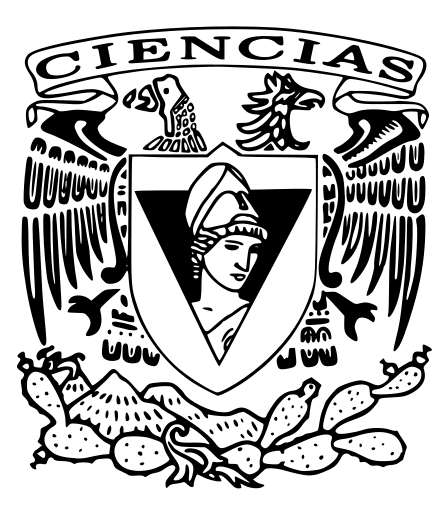
\includegraphics[width=0.5\textwidth]{escudo_f-ciencias.png}
	\vfill

% Bottom of the page
	{\large Jueves 20 de septiembre del 2018 \par}
\end{titlepage}

\pagebreak
\setlength{\voffset}{-0.75in}
\setlength{\headsep}{5pt}

%\newcommand{\ed}[2]{(#1) edge (#2)}
%\newcommand{\eee}[4]{\path [->,draw,thin] ($ (#1) !.5! (#2)$) -- ($ (#3) !.5! (#4) $);}

\newcommand{\is}[1]{V_{\{#1, x, r\}}} %Invariante de ciclo para la dem. del algoritmo

\begin{enumerate}
	%Ejercicio 1
	\item {
		Considere el siguiente algoritmo para resolver el consense en un sistema
		con $n$ procesos y con a lo más $f$ procesos fallidos.\\
		\[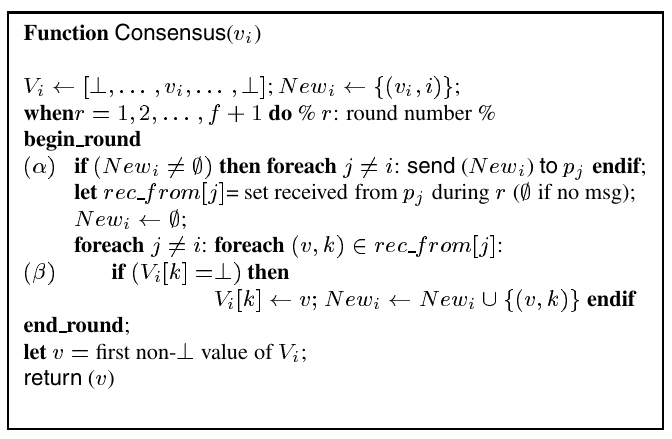
\includegraphics[width=0.5\textwidth]{consensus.png}\]

		\begin{enumerate} [label = \alph*]
			\item {
				Argumenta por qué es necesario ejecutar $f+1$ rondas para llegar a un acuedo.\\

				Los errores del modelo son únicamente de tipo crash, esto es que una vez fallado
				proceso no vuelve a funcionar.\\
				Esto significa que la cantidad de procesos vivos se queda igual o disminuye.
				Y cómo los procesos son donde está guardad la información, entonces la
				información que se puede obtener en cada ronda se queda igual o disminuye.\\
				Entonces, si en una ronda no muere ningún proceso, todos los procesos obtendrán
				toda la información disponible, y en cualquier ronda posterior habrá igual o
				menos información disponible.

				Notemos que si uno o varios procesos mueren antes de enviar cualquier
				tipo de información, entonces la información nueva que tenían se pierde.\\
				Si eran los únicos procesos vivos que tenían esa información, entonces esa
				información se puede ignorar, pues al no tenerla nadie es como si nunca
				hubiera existido. \\
				Si la información la tiene otro proceso que no ha muerto,
				entonces durante esa misma ronda el otro proceso habrá enviado esa información
				a todos los demás.\\
				De cualquier manera, la muerte de los procesos no causa inconsistencias en
				el resultado final, pues todos siguen recibiendo la misma información.\\
				Lo que puede causar inconsistencia en la decisión, es que un proceso
				muera mientras está enviando información que sólo ese proceso tiene.\\
				Esto pasa porque parte de los procesos tienen información que la otra
				parte no tiene.\\

				Entonces siempre y cuando haya una ronda donde algún proceso muera antes
				de enviar algo o nunca muera, entonces al final todos los procesos obtendrán
				la misma información, por lo que se llega a un consenso.\\
				Entonces en el caso extremo en cada ronda mueren procesos mientras están
				enviando infrmación, y el caso que requiere más rondas es cuando exactamente
				un proceso muere de esta manera cada ronda.\\
				Entonces después de $f$ rondas es posible que en cada ronda
				un proceso con nueva información haya muerto mientras enviaba la información
				a otro proceso, por lo que algunos procesos tendrían más información que otros.\\
				Como ya murieron $f$ procesos, entonces ya no puede moriri más procesos.
				Al realizar otra ronda, aseguramos que en esa ronda ningún proceso
				va a morir, y todos lor procesos vivos obtendrán toda la información
				disponible es esa ronda. Entonce todos tendrán la misma información y
				podrán llegar a un consenso.\\
			}
			\item{
				Modifica el algoritmo de la figura 1 para resolver el consenso en
				$min(t+2, f+1)$ donde $t$ es la cantidad de procesos que fallan en la
				ejecución.
			}
			\item{
				Muestra una ejecución para 4 procesos donde se ejecutan el máximo de
				rondas del algoritmo propuesto.
			}
			\item{
				Muestra una ejecución para 4 procesos donde se ejecuten el mínimo de
				rondas del algoritmo propueesto.
			}
		\end{enumerate}

	}



	%Ejercicio 2
	\item {
		Sean $A$ y $B$ dos procesos conectados por dos canales unidireccionales.
		La secuancia $G_t$ en el tiempo $t$ corresponde a $m_1, ..., m_k, n_1, ..., n_l$
		donde los $m_i$ corresponden a los mensajes enviados de $A$ hacia $B$ y $n_i$
		los enviados de $B$ a $A$, donde $k_1$ es el mensaje más reciente enviado
		por el canal.

		\begin{enumerate} [label = \alph*]
			\item {
				¿Qué cadenas de bits no son válidas al ejecutar el protocolo?
			}
			\item{
				¿Cuándo hay un cambio de bits en la coloración?
			}
			\item{
				Ejecuta el protocolo de forma que en la coloración hayan al menos 4 unos.
			}
		\end{enumerate}

	}

	\item{
		Escribe un resumen de la clase y plática impartidas por Michel Raynal.
	}

\end{enumerate}
\end{document}
